% !TEX root =  ../main.tex
\section{Oversubscription}

\subsection{Definition}

\subsubsection{Signature} \cstr{oversubscription(s : set<server>, r : string, x : number)}

\begin{itemize}
\item \cstr{s} : a non-empty set of servers
\item \cstr{r} : a resource identifier such as \cstr{mem}, \cstr{ucpu}, \cstr{pcpu} to identify the physical memory,
the computational capacity, the physical CPUs, respectively.
\item \cstr{x} : a positive percentage
\end{itemize}

The \cstr{oversubscription} constraint ensures the online servers in \cstr{s} have for each hosted VM, 
an amount of free resources at least equals to a given factor of a physical resource.
Servers not in the \st{Online} state and VMs not in the \st{Running} state are ignored.

\classification{oversubscription}{datacenter administrator}{Resource allocation}{Resource management}

\subsubsection{Usage}

The memory is usually considered as the bottleneck that limitooor the servers hosting capacity.
Originally, the memory was not shareable between the VMs so their cumulated requirement shall not exceed the servers capacity. Hypervisors such as Xen~\cite{xen-memory-sharing} or VMWare~\cite{vmware-memory-sharing} now provide sharing systems to oversubscribe the memory. 
The datacenter administrator can then use \cstr{oversubscription} constraint to control this sharing. With a factor greater than 100\%,
a server can host simultaneously VMs with a cumulated memory usage that exceed its capacity. A high factor increases the hosting capabilities of the servers but may alter the VMs performance due to the overhead of the memory sharing system.

It is also accepted to oversubscribe the physical CPUs (PCPUs) of a server. Each VM uses one or more virtual CPUs (VCPUs) and for the maximum performance, each VCPU should be mapped to a dedicated PCPU. In practice, multiple VCPU are mapped to a same PCPU when the performance overhead is acceptable.
In 2010, The Virtual Management Index reported an oversubcription ratio of 200\%: each PCPU is allocated to 2 VCPUs on average.~\cite{vmi}

Finally, a VM is usually an instance of a given template that define the maximum amount of computational resources (UCPU) it can consume. To increase the hosting capacity of the servers, the resource are often allocated dynamically, on demand,
rather than statically\cite{pMapper,violin,bobroff2007dynamic,entropy-vee09}. It is however not desirable to place too many VMs that currently consume a few uCPU on a single server as it increases the chances of having a saturated server if the VMs simultaneously increase their uCPU demand. One solution to control this oversubscription is to ensure to each of the VMs a given percentage of its maximum uCPU resource usage. For example, the datacenter administrator may use one \cstr{oversubscription} constraint and an oversubscription ratio of 80\% to ensure each server must be able to provide each of the VMs it hosts 80\% of the VM's maximum uCPU usage, even if its current demand is inferior. 

\subsubsection{Example}

Figure~\ref{fig: oversubscription} depicts a sample reconfiguration between a source and a destination configuration where each server provides 8 unit of CPU and 7 unit of memory resources to VMs. The rectangles of the VMs denotes their maximum requirements while the grey part denotes their usage. During the reconfiguration, the following \cstr{oversubscription} constraints were considered:

\begin{figure}[htb]
\centering
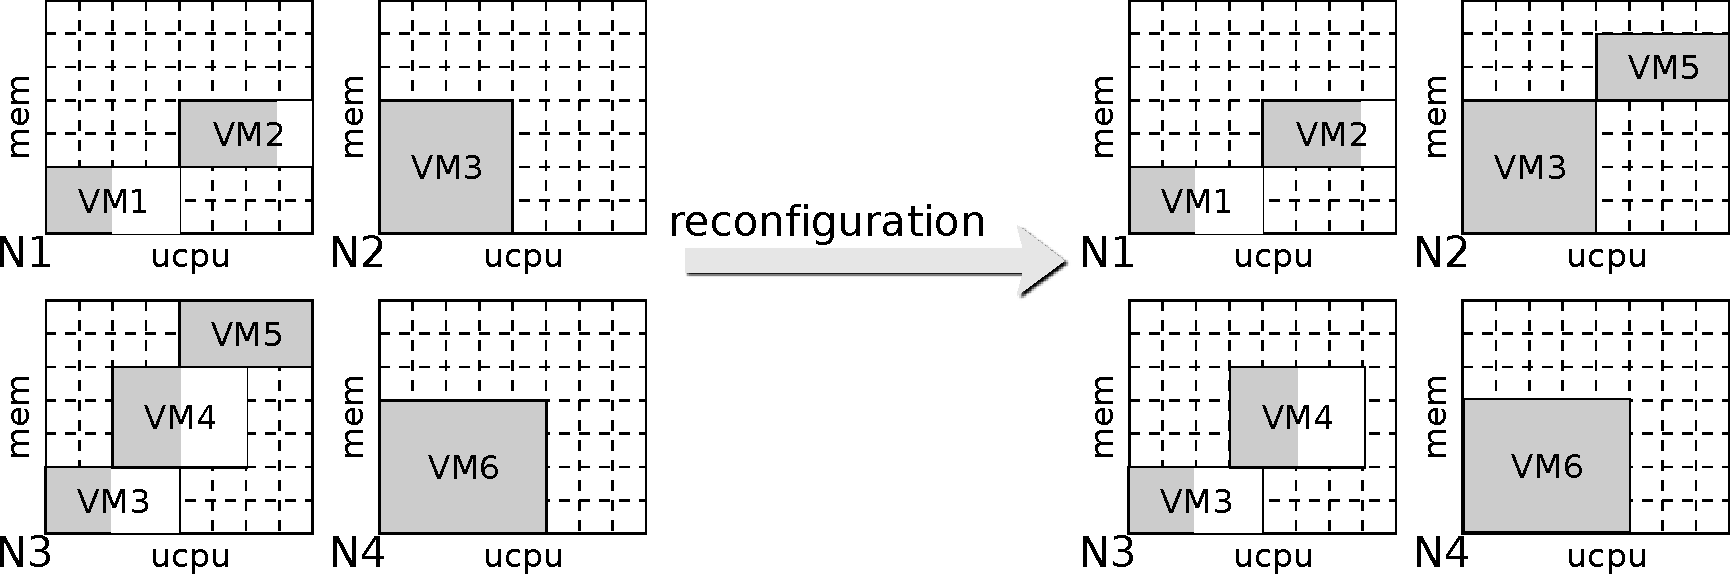
\includegraphics[width=\textwidth]{img/oversubscription}
\caption{A reconfiguration motivated by \cstr{oversubscription} constraints.}\label{fig: oversubscription}
\end{figure}


\begin{itemize}
\item \cstr{oversubscription(\{N1,N2\},"ucpu", 100\%)}. This constraint was satisfied in the source configuration
as each of the hosted VMs has enough UCPU resources to satisfy its maximum usage. The constraint is still
satisfied in the destination configuration despite the relocation of \cstr{VM5} to \cstr{N2}.

\item \cstr{oversubscription(\{N3, N4\},"ucpu",66\%)}. This constraint was not satisfied in the source configuration.
\cstr{VM3} and \cstr{VM4} were consuming 50\% of their maximum UCPU resources allowed but the presence
of \cstr{VM5} disallows them to be able to consume the required 66\%. The reconfiguration process
fixed that violation by relocating \cstr{VM5} to \cstr{N3}. As a result, \cstr{VM3} and \cstr{VM4} are ensured to be
able to consume at least 66\% of their maximum allowed. In practice, there will be able to consume 100\%.

\end{itemize}


\fullVersion{
\subsection{Model}

\subsection{Violation Detection}

\subsection{Availability}

\subsubsection{In {\btrp}}
}

\subsection{See also}

\subsubsection{Related Constraints}
\begin{itemize}
\item \cstrref{preserve}: A constraint to control the resource allocation
at the VM level.
\item \cstrref{singleCapacity}: A constraint to control the resource available on servers.
\end{itemize}

\printListOfInheritance{oversubscription}